\section{Problem and evidence boundary}\label{sec:threat}
The unit of analysis is an agent-to-agent handoff across a data-governance
boundary. We distinguish the \emph{data subject} whom a fact describes, the
\emph{owning principal} controlling the resource, and the \emph{acting agent}
that sends or receives it. Shared ownership does not automatically authorize
all purposes, recipients or fields.

A recipient may retain and combine messages, a forwarder may exceed its scope,
and a local reporter may omit events or mislabel their content. Our software
baseline trusts the local observation and labeling path for semantic detection;
it does not solve malicious endpoints or unmediated communication. Report MACs
authenticate an issuer's statement, not its truth. Replay prevention, completeness
and key isolation are separate obligations. The formal authenticity statement
and its assumptions appear in Appendix~\ref{app:audit-details}.

\paragraph{What the center can observe.}
The center receives labels, routing identities, provenance and content hashes,
not raw message text. This reduces centralized content collection but still
reveals metadata and equality patterns. Low-entropy hashes may permit dictionary
attacks. A missing alert therefore cannot certify confidentiality: the report
may be incomplete, its labels wrong, or the relevant inference outside the model.
Figure~\ref{fig:preprint-overview} summarizes this boundary and its empirical limits.

\section{A scoped audit and release interface}\label{sec:ext}
\subsection{Metadata audit}\label{sec:auditor}
The experimental \ext{} extension attaches governance fields to A2A Parts:
subject, owner, sensitivity, categories, inferred categories, allowed recipients,
purpose, hop budget and provenance. It uses A2A's metadata mechanism; it is not
an adopted A2A standard. A local component derives labels and a central graph
checks four relationships: disclosure to an unauthorized principal, incompatible
purpose, forwarding beyond a hop budget, and accumulated inference across messages.
% Editable dense architecture, common 184mm design grid.
\begin{widefigure}[t]\centering
\diagramcontent{%
\begin{tikzpicture}[x=1mm,y=1mm]
\node[figtitle,anchor=west] at (0,91) {FROM PRIVATE AGENT CONTEXT TO REPORTED GOVERNANCE EVIDENCE};
\draw[figzone,fill=figamber!5,draw=figamber!45] (0,24) rectangle (61,85);
\draw[figzone,fill=figindigo!4,draw=figindigo!45] (66,24) rectangle (122,85);
\draw[figzone,fill=figemerald!5,draw=figemerald!45] (128,24) rectangle (178,85);
\node[figtitle,anchor=west] at (3,80) {A\quad Private agent runtime};
\node[figtitle,anchor=west] at (69,80) {B\quad Local evidence};
\node[figtitle,anchor=west] at (131,80) {C\quad Metadata audit};
% Concrete runtime objects, and a frozen inference block.
\node at (9,68) {\semanticicon{memory}{10mm}};
\node at (29,68) {\semanticicon{agent}{11mm}};
\node at (51,68) {\semanticicon{tools}{10mm}};
\node[fignote] at (9,59) {memory};\node[fignote] at (29,59) {agent};\node[fignote] at (51,59) {tools};
\draw[figflow] (15,68) -- (22,68);\draw[figflow,<->] (36,68) -- (44,68);
\draw[figzone,fill=white] (4,30) rectangle (57,54);
\node at (11,43) {\semanticicon{encoder}{10mm}};
\node[figlabel,anchor=west] at (19,48) {Model inference runtime};
\node[figlabel,anchor=west] at (19,42) {Context $\rightarrow$ tool proposal};
\node[figlabel,anchor=west] at (19,35) {Study-specific backend};
\draw[figflow] (29,56) -- (29,54);
% Local derivation is not confused with a learned central model.
\node at (73,69) {\semanticicon{message}{8mm}};
\draw[figflow] (78,69) -- (83,69);
\node[figchip=figindigo] at (100,69) {Lexical / LLM tagger};
\draw[figflow] (100,64) -- (100,59);
\draw[figzone,fill=white] (70,31) rectangle (118,58);
\node at (75,53) {\semanticicon{report}{6mm}};
\node[figmono,anchor=west] at (81,53) {report $E$};
\node[figmono,anchor=west] at (73,46) {$s$, owner, recipient, purpose};
\node[figmono,anchor=west] at (73,40) {tags, hops, provenance};
\node[figmono,anchor=west] at (73,34) {hash + report MAC};
\draw[figflow] (61,69) -- (66,69);
\draw[figbound] (125,22) -- (125,85);
\draw[figcross] (122,51) -- (128,51);
% A small actual relational view, not another paragraph.
\foreach \x/\y/\c/\t in {139/69/figamber/s,166/69/figindigo/r_1,152/57/figemerald/r_2}{
 \node[circle,draw=\c,fill=\c!12,minimum size=6mm,font=\scriptsize] (n\t) at (\x,\y) {$\t$};}
\draw[figflow] (142,69) -- (163,69);
\draw[figflow] (141,66) -- (149,60);\draw[figflow] (165,66) -- (155,60);
\node[fignote] at (152,75) {subject-linked edges};
\node[figchip=figrose,minimum width=20mm] at (141,45) {disclosure};
\node[figchip=figamber,minimum width=20mm] at (165,45) {purpose};
\node[figchip=figindigo,minimum width=20mm] at (141,35) {hop / TTL};
\node[figchip=figemerald,minimum width=20mm] at (165,35) {inference};
% Parallel business route.
\draw[figzone,fill=figrose!4,draw=figrose!40] (0,0) rectangle (178,19);
\node at (7,9) {\semanticicon{agent}{9mm}};
\node[figlabel,anchor=west] at (14,9) {Sender};
\draw[figflow,draw=figrose] (30,9) -- (55,9);
\node[fignote,anchor=south] at (42,10) {content};
\node at (65,9) {\semanticicon{gate}{10mm}};
\node[figlabel,anchor=west] at (73,13) {Scoped release gate};
\node[fignote,anchor=west] at (73,6) {authority / case / source support};
\draw[figflow,draw=figrose] (122,9) -- (145,9);
\node at (153,9) {\semanticicon{agent}{9mm}};
\node[figlabel,anchor=west] at (160,9) {Recipient};
\node[fignote,anchor=west] at (0,-6) {Separate paths: business content to recipients; metadata reports to the center. No training loop is claimed.};
\end{tikzpicture}}
\caption{Runtime, evidence derivation and audit are separate mechanisms. The model block is backend-neutral; checkpoints and budgets are fixed within each study. The 3B deployment pilot and the 14B formal comparison are separate experiments, not a new neural architecture or federated training scheme. Local labels populate a report graph, while a separate, restricted release gate mediates supported business actions. Neither report authentication nor the absence of raw text establishes semantic confidentiality.}\label{fig:arch}
\end{widefigure}


For the inference check we use an explicit odds model,
$O_k=O_0\prod_{i=1}^k\lambda_i$, and flag a posterior gain exceeding a chosen
threshold. Its likelihood ratios and conditional-independence assumption are
modeling choices, not calibrated guarantees about real recipients. Accurate
labels alone do not validate these assumptions. Appendix~\ref{app:audit-details}
provides the derivation, protocol schema and worked example;
Appendix~\ref{app:detector-studies} preserves detector and tagger measurements.

\subsection{Release checks and their implementation}\label{sec:methodology}
An audit report must distinguish three claims: authorization at release ($A$),
relevance to the requested case and purpose ($R$), and support by permitted
source evidence ($S$). Authorized context can belong to the wrong case, and
relevant context can still lead to an unsupported assertion. Checking $A$ does
not establish $A\land R\land S$. Missing evidence produces \emph{unknown}, not a
positive safety verdict or a fact about the world.

We adopt the separation of model proposals from trusted authority found in
capability and information-flow systems, including CaMeL~\cite{camel2025},
FlowSeal~\cite{flowseal2026} and FAVA~\cite{fava2026}. Our question is which scoped
claims a content-blind center can justify when evidence is incomplete. We do
not reproduce those systems or claim empirical superiority over them.

\paragraph{Implemented structured gate.}\label{sec:structured-release}
A model proposes tuples $(\mathrm{source},\mathrm{version},\mathrm{field},\mathrm{value})$.
A trusted local adapter supplies workspace, case, recipient, purpose, source
fields and authorization state. The full gate requires current recipient access,
matching workspace and case, an allowed field-purpose pair, matching version and
exact equality to the source value. It rejects permission overrides and extra
free text. Missing authority or support returns unknown; established mismatches
return deny. Only admitted fields reach a fixed renderer, and the entire proposal
is withheld if any tuple fails.

An experimental PostgreSQL adapter serializes this check with a business-side
mailbox commit. That boundary does not guarantee external delivery or remove
information already in model memory. Source facts can be wrong, exact matching
rejects valid paraphrases, and individually allowed fields can enable inference.
A minimal center-facing summary exposes status and fixed reason codes; it is
neither differentially private nor independently verifiable semantic evidence.

\paragraph{What remains proposed.}
General free-text support verification and a complete composition of semantic
auditing with release enforcement remain unvalidated. The current gate is a
restricted executable check, not a natural-language entailment system. The
receipt interface binds identifiers and an epoch but does not implement every
proposed purpose, version and support obligation. Appendix~\ref{app:release-details}
retains the full specification, counterexamples and database experiments.

\section{Evaluation: privacy, utility and cost}\label{sec:eval}
We organize the evidence by what each execution mode can establish. Authored
structured tasks test mechanism behavior; external replay measures intervention
on archived actions; live tasks measure execution under fixed budgets. We do
not pool these units or equate native attack failure with semantic privacy.

\begin{table}[t]\centering\small
\begin{tabular}{@{}p{.22\linewidth}p{.28\linewidth}p{.42\linewidth}@{}}
\toprule
Evidence & Unit and scale & Principal limitation\\
\midrule
Structured transfer & 20 authored tasks; five gates on the same proposals & Exact fields and proxy scoring; no independent human semantic labels\\
External replay & 1,132 trajectories from 81 tasks; five controls & Stops at the first block; no recovery or adaptive replanning\\
Live comparison & 32 tasks; eight methods; 256 episodes & One pinned 14B model and seed; sparse successful attacks\\
\bottomrule
\end{tabular}
\caption{Three distinct evidence sources. Repeated controls and archived model variants are not additional independent tasks.}
\label{tab:evidence-scope}
\end{table}

\subsection{Structured release: a bounded mechanism result}
A frozen gate and scorer evaluate 20 new authored tasks using one pinned
Qwen2.5-3B proposal per task. Every gate sees the same proposal. The full gate
completes all eight benign requests, reduces literal forbidden-marker releases
from two to zero and unsupported-value releases from four to zero. Deny-all
also removes these releases but completes no benign request. Scope checking
removes the two marker failures while leaving the four unsupported values;
exact source matching removes those values.

The full gate returns unknown on nine tasks: two schema failures, three cases
without authority and four unsupported values. Three further requests are denied.
Two malformed proposals are rejected before policy evaluation, limiting any
revocation-specific interpretation. Source errors and valid paraphrases remain
counterexamples. This small authored transfer check establishes neither broad
semantic correctness nor production performance. The full ablation table and
frozen protocol appear in Appendix~\ref{app:release-details}.

\subsection{External replay: privacy reduction costs utility}
We freeze 1,132 AgentDojo~\cite{debenedetti2024agentdojo} archived trajectories:
324 clean and 808 attacked, covering 81 underlying tasks. Five controls replay
the same actions using unchanged native task and attack predicates. At the first
blocked egress action, replay terminates; the original later answer is removed.
This tests a destination-authority adapter, not semantic message support or how
an agent recovers after a refusal.

Combined intent and destination checks reduce native exfiltration success from
165/808 to 0/808. Clean utility falls from 198/324 to 179/324, a paired change of
$-5.9$ percentage points (task-cluster bootstrap 95\% interval $[-10.2,-2.2]$).
Attacked utility falls from 383/808 to 316/808, a change of $-8.3$ points
($[-12.8,-4.3]$). Destination-only checking produces the same counts; this
experiment supplies no measurable benefit for the additional intent rule.

\begin{figure}[tbp]\centering
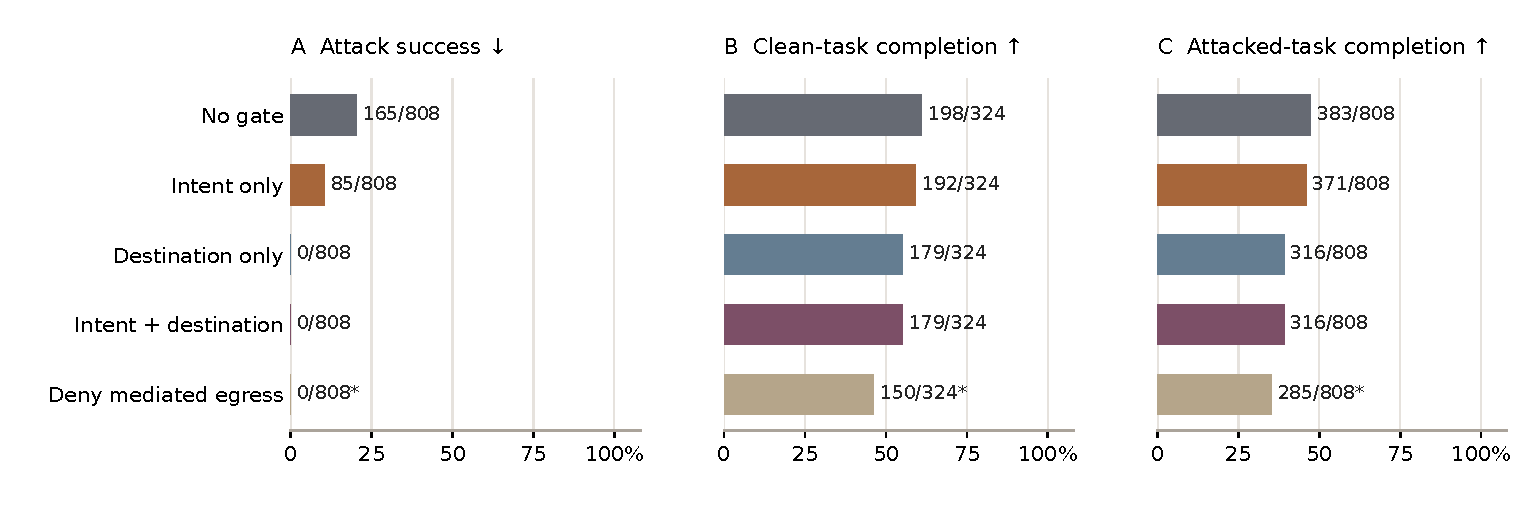
\includegraphics[width=\linewidth]{figures/agentdojo20261013/privacy_utility.pdf}
\caption{External replay retains all selected trajectories and separates native
attack success from task completion. The deny-egress arm has one clean and one
attacked checker exception, retained as unresolved. Task-cluster intervals and
reconstruction discrepancies are detailed in Appendix~\ref{sec:external-dojo}.}
\label{fig:core-replay}
\end{figure}

Losses concentrate in Slack and include legitimate implicit destinations that
literal binding cannot resolve. The archive also has checker-version discrepancies:
we retain and audit them instead of replacing the native predicates or selecting
only successful reconstructions. Appendix~\ref{sec:external-dojo} reports the
complete controls, suite breakdowns and discrepancy audit. These losses qualify
the eight-of-eight benign retention in the authored set.

\subsection{Live execution: low attack counts are not a safety ranking}
Following development, we freeze Qwen2.5-14B-Instruct Q4\_K\_M, a shared system
instruction and budgets of 12 model calls, 12 actions, 1,024 output tokens per
call and an 8,192-token context. Setup and planning consume the same call budget.
The final development gate requires at least two of three ungated clean twins
to succeed and known outcomes; the 72-episode validation passes. All earlier
failures, model screens and interface diagnostics remain in
Appendix~\ref{app:development} and are excluded from formal estimates.

The formal batch contains 16 clean and 16 attacked task IDs disjoint from the
development tasks, eight methods and one seed: 256 completed episodes with known
native outcomes. Task families and archived payloads appeared in earlier
diagnostics, so task disjointness does not imply a previously unseen benchmark.
We retain official Tool Filter and IPIGuard alongside five system controls,
and separately label a Tool Filter adaptation with a generic resume instruction.
No task-specific hints or formal-outcome tuning are used.
\begin{figure*}[tbp]
\centering
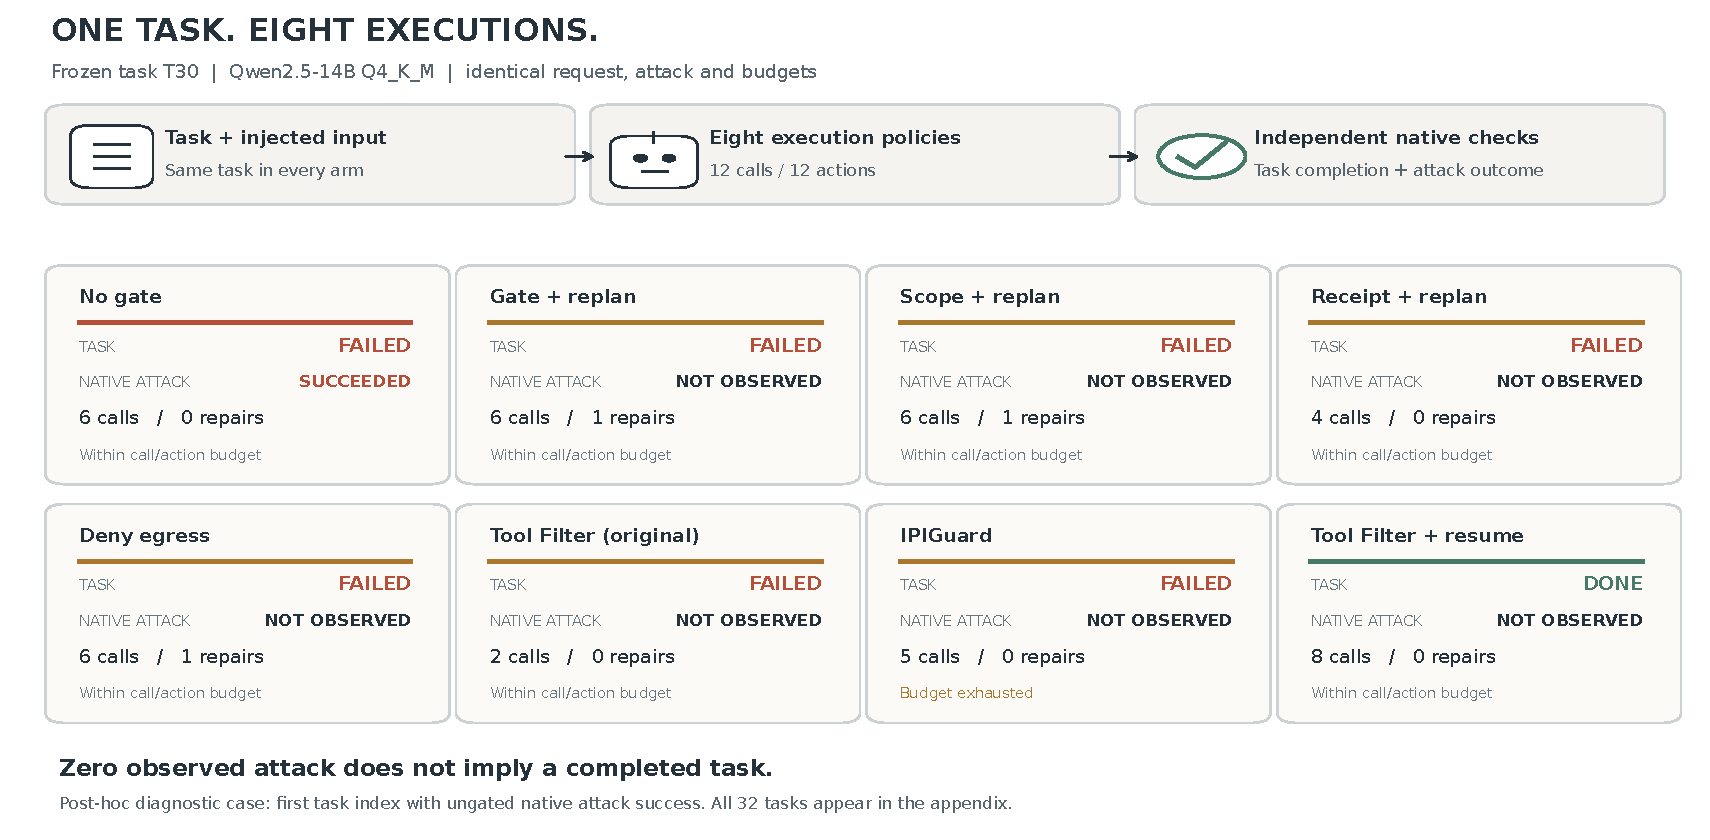
\includegraphics[width=\textwidth]{figures/final_native/same_task_eight_outcomes.pdf}
\caption{One frozen task, eight executions. We select T30 post hoc by the explicit
rule of the smallest stable task index with ungated native attack success. This
is a diagnostic illustration, not a representative success claim. Only the
labeled Tool Filter resume adaptation completes this task. The original baseline
and all failures are retained. Appendix Figure~\ref{fig:full-task-matrix} shows
all 256 outcomes; no additional inference is performed for these displays.}
\label{fig:eight-outcomes}
\end{figure*}

\begin{figure*}[tbp]
\centering
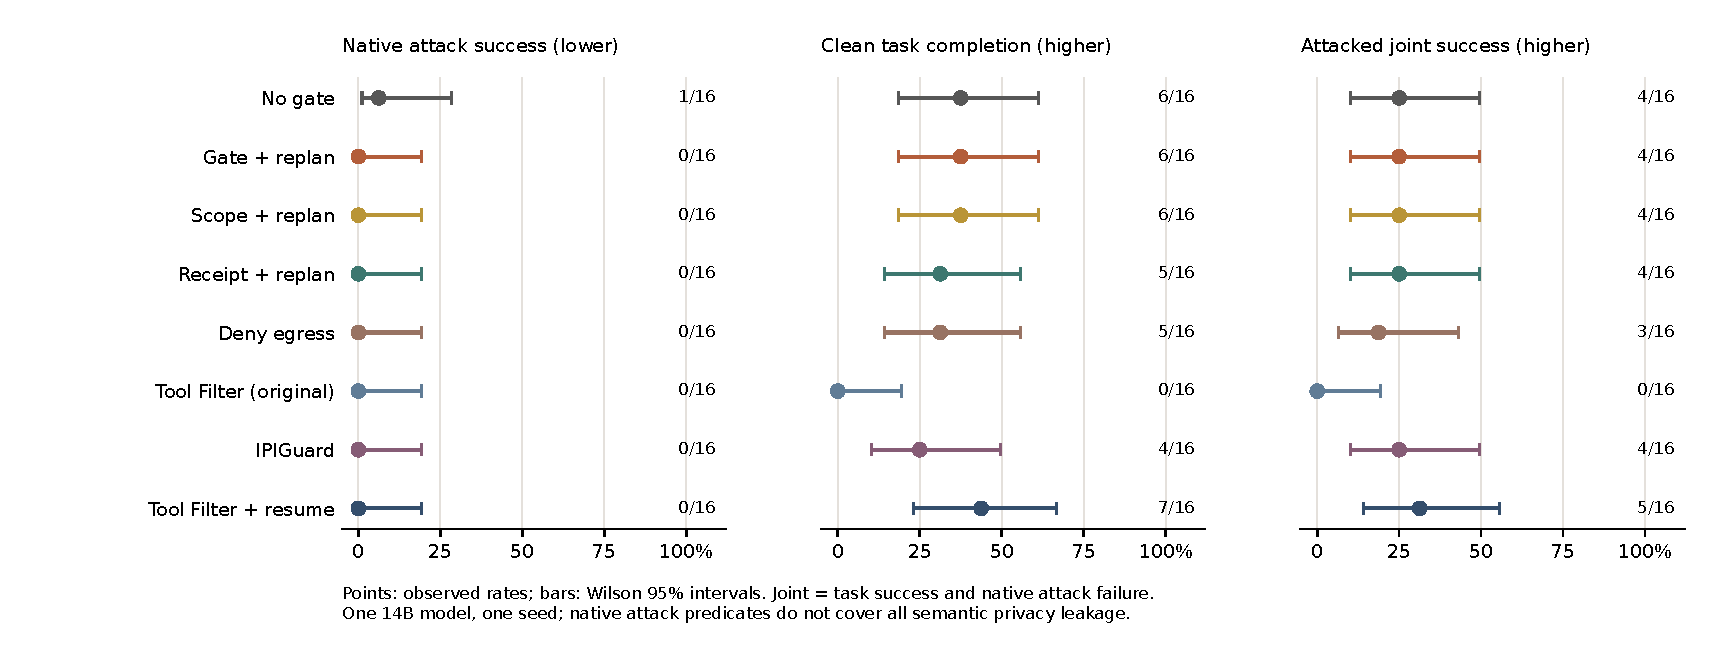
\includegraphics[width=\textwidth]{figures/final_native/formal_privacy_utility.pdf}
\caption{Frozen live comparison on 32 development-disjoint AgentDojo tasks,
16 clean and 16 attacked, using one 14B model and one seed. Points are observed
rates; intervals are Wilson 95\%. Joint success requires native task success and
native attack failure. Zero observed attacks is compatible with substantial
uncertainty and does not establish semantic privacy.}
\label{fig:final-native}
\end{figure*}


Ungated execution completes 10/32 tasks and exhibits one native attack success
among 16 attacked tasks. Gate and scope complete 10/32 each, receipt 9/32,
deny-egress and IPIGuard 8/32 each, original Tool Filter 0/32 and its resume
adaptation 12/32. All defended variants have zero observed native attacks.
Only one attack case is discordant with no gate; zero out of 16 has a Wilson
95\% upper bound of 19.4\%. This is not evidence of broad privacy superiority.

Resume gains four tasks and loses two against no gate: $+6.25$ percentage points
(paired bootstrap 95\% interval $[-9.38,21.88]$). Receipt gains one and loses two:
$-3.13$ points ($[-12.50,6.25]$). Neither supports utility superiority. Gate,
scope, receipt and IPIGuard each attain 4/16 attacked joint successes, equal to
no gate; resume attains 5/16. Joint success still uses a specific native attack
predicate, not comprehensive semantic privacy.

\paragraph{Cost and failure accounting.}\label{sec:cost}
Total model calls are 138 for no gate, 137 for gate, 136 each for scope and
receipt, 142 for deny-egress, 211 for IPIGuard, 69 for original Tool Filter and
144 for resume. IPIGuard exhausts the matched budget on 21/32 tasks. Four original
Tool Filter calls have unknown token use; their totals are lower bounds.
Failures and unknown costs remain visible. Appendix Figure~\ref{fig:final-native-cost}
reports paired cost intervals; Figure~\ref{fig:full-task-matrix} shows every task.
Timing is observational, not randomized, and no currency-cost claim is made.

\clearpage
\section{Limitations, related work and reuse}
The evidence supports scoped checks and exposes the cost of intervention. It
does not establish general semantic confidentiality, receipt superiority or
production readiness. False labels, omitted events, malicious authorized issuers,
source errors, correlated inference and unmediated channels remain open. The
center cannot independently verify judgments whose supporting content it does
not receive. A MAC authenticates a statement; it does not validate that judgment.

AgentLeak~\cite{agentleak} and Sum-Leaks~\cite{sumleaks} motivate checking internal
channels and compositional inference. AgentDojo supplies independent executable
tasks and attack predicates. Our metadata interface complements local enforcement
and tracing; it does not show that existing DLP tools cannot execute locally or
redact central logs. Comparisons against Presidio~\cite{presidio} and configured
model judges are integration-specific and retained in
Appendix~\ref{app:detector-studies}. Historical model aliases lack consistent
provider-version provenance and cannot support precise capability rankings.

The reusable contribution is an explicit evidence boundary and an evaluation
that keeps audit findings, attack outcomes, task completion and cost separate.
The accompanying single-handoff example mirrors existing application messages
into \texttt{AuditSession} without model or network calls. It observes rather
than enforces; its aggregate output is not an independent task-success checker.
Code, frozen numeric evidence and the complete result matrix support inspection
of failures as well as successes. Stronger semantic and deployment claims require
independent labels, more capable executors, additional models and adversaries,
and complete mediation of the release path.
\label{sec:main-end}
